\documentclass[12pt,a4paper]{article}
\usepackage[utf8]{inputenc}
\usepackage{amsmath,enumitem,amsfonts,amssymb,graphicx}
\usepackage{multicol}
\usepackage{sectsty}
\graphicspath{ {./} }
\usepackage{scrextend}

\usepackage[%
    left=1.0in,%
    right=1.0in,%
    top=0.8in,%
    bottom=1.0in,%
]{geometry}%

\sectionfont
{\fontsize{14.4}{12}\selectfont}
\title{\textbf{Principles of AI Planning
		\\{\Large Exercise Sheet 5}}}
\date{29.11.2019}

\makeatletter
\renewcommand{\@maketitle}
{
	\newpage
	\null
	\vskip 2em%
	\begin{center}%
		{\LARGE \@title \\ \par}%
	\end{center}%
	\par
} \makeatother


\begin{document}
	\begin{flushleft}
		Authors:\\
		Erick Rosete Beas | er165@uni-freiburg.de\\
		Jessica Lizeth Borja Diaz | jb986@uni-freiburg.de\\
	\end{flushleft}
	{\let\newpage\relax\maketitle}
	\begin{center} 
		\large 29.11.2019 
	\end{center}

\hfill\break
\section*{Exercise 5.1: A* search}
	\textbf{a) Solve the puzzle with the A* algorithms}\\
	Using the heuristic as a tie breaker, favoring lower h values,
	we get the following tree.
	Where we find the optimal solution as the heuristic is admissible and
	because every other f value in the heap is bigger or equal to five.
	\begin{center}
		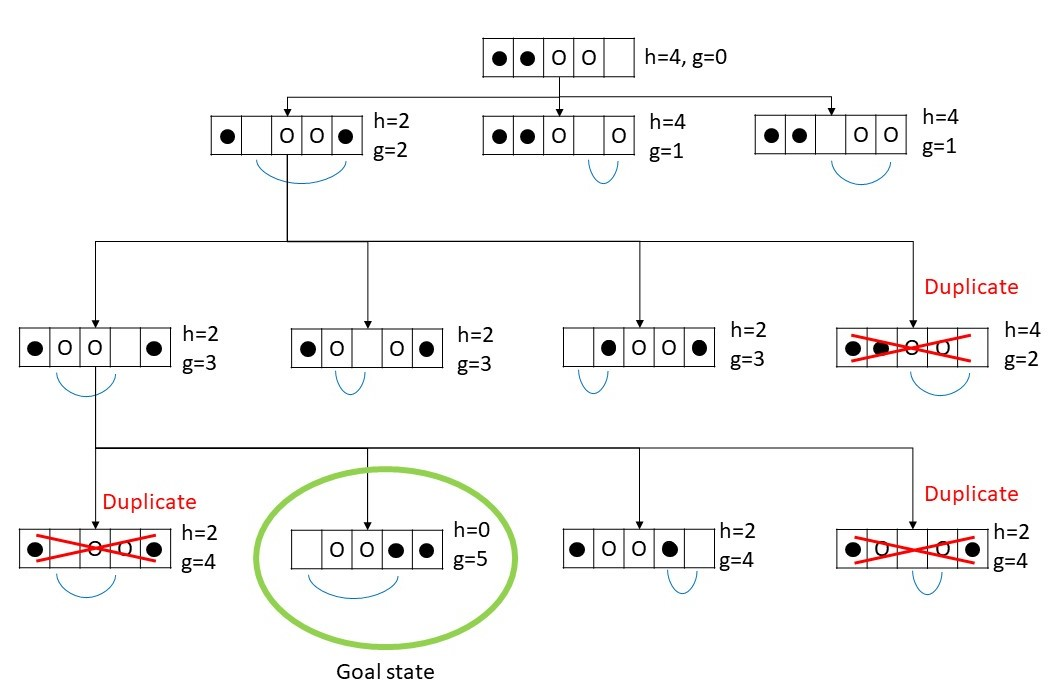
\includegraphics[scale=0.4]{A_star_0.jpg}\\
	\end{center}
	\textbf{b) show that h is admissible}
	\begin{addmargin}[1em]{1em}% 1em left, 2em right
		\quad Given an initial state with a black tile to the left of a white
		tile, the only way that a black tile can reach the goal state is if
		it jumps this white tile. \\
		If it jumps through the white tile, this movement always causes a cost equal or bigger to 1 per white tile at the right side, this can be seen because the cost were established as following.\\
		- The cost of jumping over one tile is 1.\\
		- The cost of jumping over two neighboring tiles is 2. \\
		Additionally it is not always equal, as movements without jumping are allowed and is not always possible to jump the tiles without additional movements.\\
		This means that the sum of cost operations required for the black tile to reach a goal state,
		is \textbf{at least} the number of white tiles to the right, which is 
		precisely our heuristic. Therefore $h(s) \leq h^*(s) $
		and in consequence the heuristic is \emph{admissible}
	\end{addmargin}

%%%%%%%%%%%%%%%%%%%%%% Exercise 5.2 %%%%%%%%%%%%%%%%%%%%%%%%%%%%%
\section*{Exercise 5.2: Enforced hill-climbing}
\begin{enumerate}[label=\alph*)]
	\item \textbf{For each invocation of the 
			\texttt{improve} procedure, specify
			the state after improvement by giving the new coodinates}\\
	The given coordinates will be expressed as H(Horizontal Coordinate, Vertical Coordinate), G(Horizontal Coordinate, Vertical Coordinate), where H is the position of Hansel and G is the position of Gretel\\
	\[h(\sigma_0) = 5 \qquad \sigma_0 = H(1,2), G(4,4) \]
	\[h(\sigma_1) = 4 \qquad \sigma_1 = H(1,3), G(4,4) \]
	\[h(\sigma_2) = 3 \qquad \sigma_2 = H(2,3), G(4,4) \]	\[h(\sigma_3) = 2 \qquad \sigma_3 = H(3,3), G(4,4) \]	\[h(\sigma_4) = 1 \qquad \sigma_4 = H(3,3), G(3,2) \]	\[h(\sigma_5) = 0 \qquad \sigma_5 = H(3,3), G(3,3) \]	
	\item \textbf{Record the solution plan}
	\[north_H \quad \rightarrow \quad east_H \quad \rightarrow \quad east_H \quad \rightarrow \quad east_G
	\quad \rightarrow \quad south_G \]
	\[\quad \rightarrow \quad south_G \quad \rightarrow \quad west_G \quad \rightarrow \quad west_G \quad \rightarrow \quad north_G\]
\end{enumerate}
\end{document}